rate limiting was one interesting aspect for security, as it's a way to prevent the
server from being flooded with requests. As it could stop DDOS attacks, brute force
attacks, and any other kind of attack that would require sending lot of request from 
the same IP or same user.

For the rate limiting, as we were using already a Spring backend we had a couple options
to choose from the first one was Bucket4j, which is a rate limiter that relies on token
bucket algorithm which approaches rate limiting through putting a number of tokens in a
bucket then whenever the consume or client tries to use a service it has to consume one
or more tokens from the bucket until they are depleted then the client is blocked,
the bucket is then assigned to a key which could be a user, IP address or API key ...

The second option was to use Resilience4j, which relies on creating cycles where each cycle
has a number of allowed permissions and refreshes in the beginning of each cycle, which
allows the handling of the rate limiting in a epoch fashio but it was not easy to
implement for the case of a distributed backend and not worth the trouble to adapt it
with a caching system within the Redis Database to do so, as it relied heavily on
single machines threads for the handling it does.

So we went with the former, which was implemented as a filter within the API gateway
in the Spring backend as shown figure \ref{fig:b4j}.

\begin{figure}[!htpb]
    \centering
    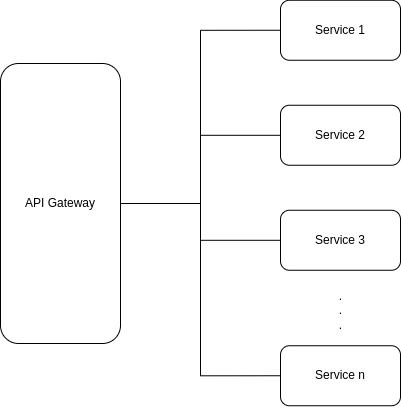
\includegraphics[width=0.5\textwidth]{images/ratelimiting.png}
    \caption{\footnotesize{Backend Gateway}}
    \label{fig:b4j}
\end{figure}


So the now the handling of services within the Java Spring backend required the passage
from API rate limiter which consisted of giving a token to the client before allowing
the request to be processed, and this requests were by default capped to a certain number
that could be modified through the configuration file of the server.

Now with the basic handling in hand, we opt for the implementation of the rate limiter
which was done in two ways, the first was to have a bucket for each user,
and the second was to have a bucket for each IP address.

Rate limiting the user was specifically setup for handling the private endpoints and that
was able to be modified by the admin to allow for more or less requests per second
depending on the user, and the rate limiting the IP address was setup for the public API.

And lastly there was the rate limiting for the login, which was individually handled for
the purpose of limiting the number of login attempts per minute to avoid possibility
of a dictionnary attacks.

